\subsection*{Измерения}

При различных углах рассеяния $\theta$, измерим спектр детектируемых на сциотилляционном счётчике, а именно, найдём на каком канале $N$ счётчика наблюдается максимум (см. таблицу 1).
По измеренным данным, построим зависимость $1/N = f(1-\cos \theta)$ (см. рис. 2).

\begin{table}
    \centering
    \caption{Зависимость номера канала $N$ от угла рассеяния $\theta$}
\begin{tabular}{c|rrrrrrrrrrrr}
% \toprule
\hline
 $N$   &  857 &  795 &  747 &  648 &  578 &  507 &  459 &  414 &  376 &  345 &  318 &  296 \\
$\theta$ &   10 &   20 &   30 &   40 &   50 &   60 &   70 &   80 &   90 &  100 &  110 &  120 \\
% \bottomrule
\hline
\end{tabular}
\end{table}




\begin{figure}[h]
    \centering
    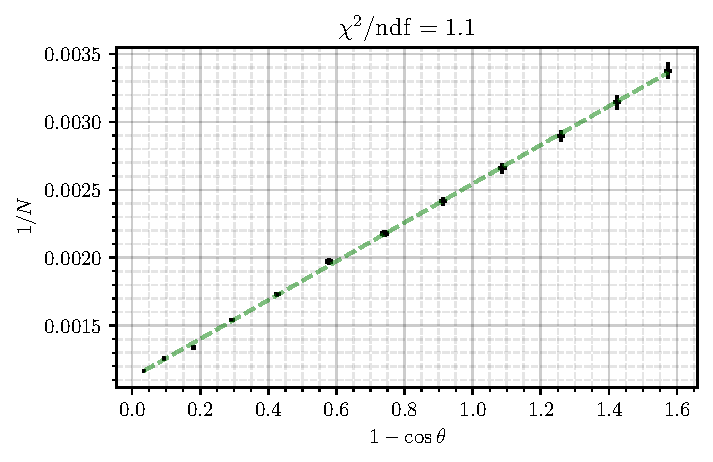
\includegraphics[width=0.5\textwidth]{figures/plot.pdf}
    \caption{Зависимость $1/N = f(1 - \cos \theta)$}
    \label{fig:1}
\end{figure}

Найдём коэффициенты линейной зависимости $f(x) = a x + b$, как $1/N = f(1-\cos \theta)$ (см. рис. \ref{fig:1}). Далее, найдём погрешность значений $N_{0}$ и $N_{90}$, исходя из
\begin{equation*}
    N_{0} = f(0) = b, \hspace{5 mm} 
    \sigma\left[N_0\right] = \sigma\left[b\right],
    \hspace{10 mm} 
    N_{90} = f(1),
    \hspace{5 mm} 
    \sigma\left[N_{90}\right] = \sqrt{\begin{pmatrix}
        1 \\ 1
    \end{pmatrix}\T \cdot \text{Cov}\, \cdot \begin{pmatrix}
        1 \\ 1
    \end{pmatrix}},
\end{equation*}
откуда находим
\begin{equation*}
    N_0 = 896 \pm 7
    \hspace{10 mm} 
    N_{90} = 393 \pm 1.
\end{equation*}
Подставляя в формулу (2), находим
\begin{equation*}
    m c^2 = E \frac{N_{90}}{N_0 - N_{90}} = (517 \pm 10) \ \text{кэВ},
    \hspace{10 mm} 
    (m c^2)^{\text{table}} = 512 \ \text{кэВ},
\end{equation*}
где, как видим, полученное значение в пределах погрешности совпадает с табличным значением для энергии покоя электронов.




% Diagram shows ...

% It is 